% This is samplepaper.tex, a sample chapter demonstrating the
% LLNCS macro package for Springer Computer Science proceedings;
% Version 2.20 of 2017/10/04
%
\documentclass[runningheads]{llncs}
%
\usepackage{graphicx}
\usepackage{hyperref}
\usepackage{subcaption}
\usepackage{float}
\usepackage{multirow}% http://ctan.org/pkg/multirow
% Used for displaying a sample figure. If possible, figure files should
% be included in EPS format.
%
% If you use the hyperref package, please uncomment the following line
% to display URLs in blue roman font according to Springer's eBook style:
% \renewcommand\UrlFont{\color{blue}\rmfamily}

\begin{document}
%
\title{Lane Detection using a combined CNN and RNN}
%
%\titlerunning{Abbreviated paper title}
% If the paper title is too long for the running head, you can set
% an abbreviated paper title here
%
\author{Shen Chen (MS)\and
Yang Liu (MS)\and
Spencer Pozder (BS/MS)}
\institute{Northeastern University}
%
\maketitle              % typeset the header of the contribution
%
\begin{abstract}
Neural networks play an important role in the area of data analytics using machine learning. One of the most successful example is the Convolutional Neural Network (CNN). By introducing multiple convolutional layers, the network can be used to classify data automatically based on features. It has become a powerful tool especially in the area of computer vision. Recently, Recurrent Neural Networks (RNN) have gathered more interest. These networks introduce connections between the neurons inside the network to let the model have a period of memory. In this project, we try to combine both of the networks' advantages and use them to do lane detection.
\end{abstract}
%
%
%
\section{Introduction}
Lane detection is an important problem in the field of autonomous driving. Traditionally, it is solved using computer vision tools and knowledge. But these tools work poorly in challenging conditions, such as when the images become blurry or dark . With the development of machine learning, researchers have started to use different machine learning models to find solutions to this problem. Chang, C. and Lin, C.~\cite{ref:1} introduced a model that uses a Support Vector Machine. It attempts to classify every pixels in the picture into lane or not lane using a Gaussian radial basis function as the kernel. But in some situations, such as when there are very large, similar color regions in the view, it will misclassify these regions as part of the lane. Juan Pablo Gonzalez and Omit Ozguner.~\cite{ref:2} introduced using decision trees to detect the obstacles in the road, and then employing the use of computer vision technology to detect the lane. However, this approach is still based on edge detection techniques primarily. In this paper, we introduce a method to detect the lane by combining both an CNN and RNN in order to overcome these shortcomings. \\
The structure of this paper is, first, we will briefly introduce CNN, RNN and others’ work that use a CNN to detect the lane. Then the dataset and labels will be showed in section 2. After that, we will discuss our architecture in section 3. Moreover, in section 4 and 5 the implementation details and results will be analyzed. Finally, we will discuss the current drawbacks and possible improvements.


\subsection{Convolutional Neural Network}
The Convolutional Neural Network is inspired by biological neurons and the animal vision contex. The neurons inside a layer are connected to the neurons in next layer. By using convolution and pooling, the training of CNN has a reasonable amount of computations for training/analysis. It is widely used in image and video processing,  natural language processing and recommendation systems. \\
In many cases, convolutional neural networks have been proven effective and it has subverted traditional computer vision field in many aspects.

\subsection{Recurrent Neural Network}
The Recurrent Neural Network is a neural network in which its neutrons have a link to the next neutrons in the graph along the sequence. RNN can then use its internal state to store the previous information, and therefore, exhibit a temporal behavior based on its memory. It is often used in handwriting recognition and speech recognition, as these problems contain features dependent on time.

\subsection{Past Research}
Much research in regard to lane detection has already been done. For example, Sandipann P. Narote, etc developed a driver assistance system (das) to provide aid or assistance to the driver while driving. Their system continuously monitors the position of the vehicle compared to the lane markers on either side~\cite{ref:3}. Jun Li, etc proposed a framework that use CNN to decide if there is a lane in sight, and then use RNN to simulate the geometry of the lane that the car is currently in~\cite{ref:4}. Yan Tian, etc introduced a method to mark lanes automatically with deep neural network~\cite{ref:5}. Mister Michael Virgo had implemented a lane detection project with a SegNet model that have 7 convolutional layers and 7 deconvolutional layers~\cite{ref:6}.

\section{Dataset}
There are many open source lane datasets available online, but many are unlabled. We chose to use the CULane dataset because it has abundant lane images taken in challenging situations like lanes in crowded traffices, at night, under shadow, having dazzling light or having no line on the road, as well as existing labels for the lanes in the images. This CULane dataset was collected by a research group at the Chinese University of Hong Kong.

\begin{figure}
\centering
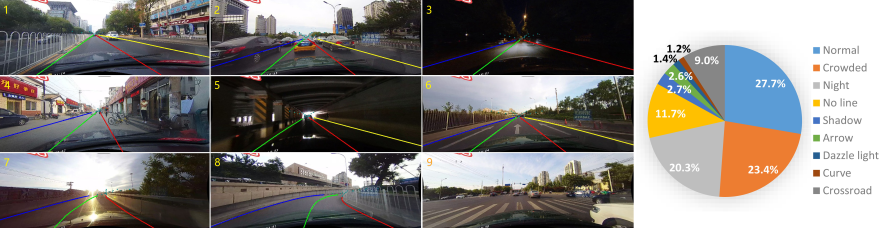
\includegraphics[width=\textwidth]{Figure1}
\caption{sample pictures from CULane dataset~\cite{ref:7}} \label{fig:1}
\end{figure}
	
In the CULane dataset, labels are given by feature points of lane boundaries in text files, and include all the lanes in sight for convenience of use. However, in our case, we are only interested in the current lane the car is in, so we first extracted the current lane information from all the lanes that are labeled in the dataset. \\

To extract the dataset into the form that we wanted, we created another set of black background images and ploted all the feature points of the lanes onto these black “curtains”. Then, we used opencv~\cite{ref:9} to connect all the boundaries to lines and fill the polygons as lane labels.

\begin{figure}[H]
\begin{subfigure}{.5\textwidth}
  \centering
  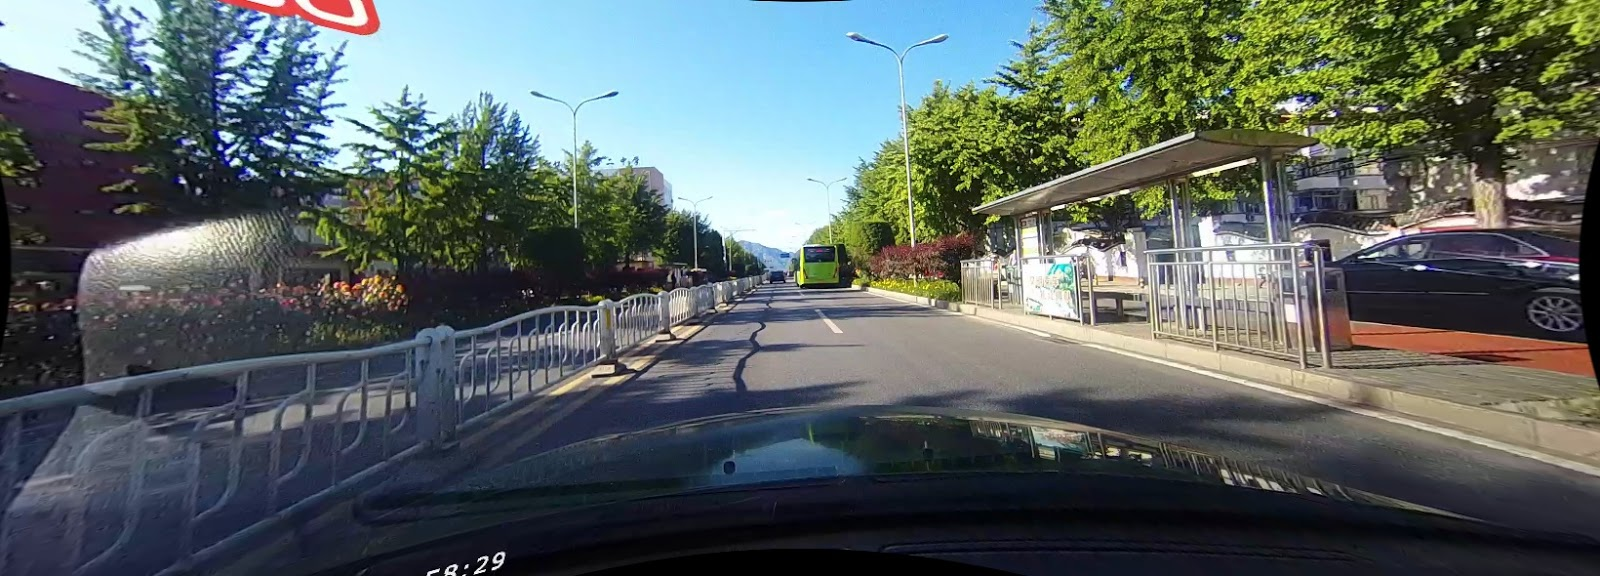
\includegraphics[width=.8\linewidth]{Figure2a}
  \caption{Original image}
  \label{fig:2sfig1}
\end{subfigure}%
\begin{subfigure}{.5\textwidth}
  \centering
  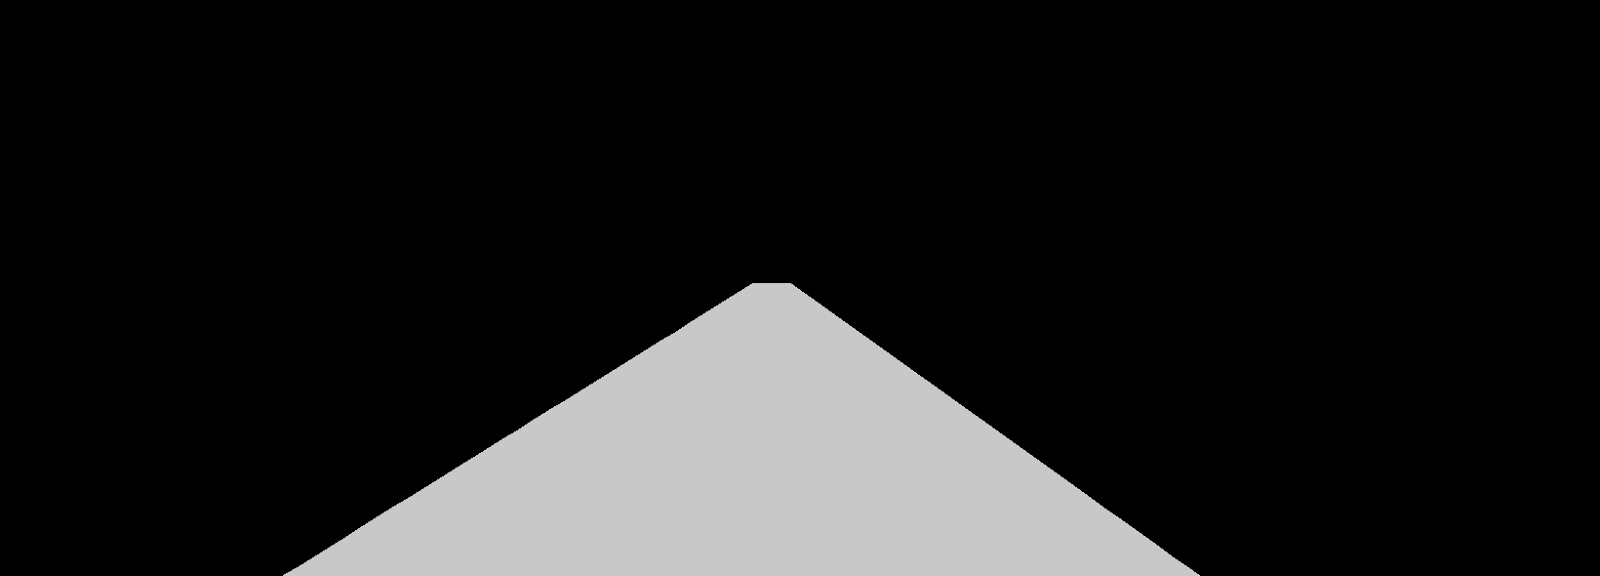
\includegraphics[width=.8\linewidth]{Figure2b}
  \caption{Corresponding lane label}
  \label{fig:2sfig2}
\end{subfigure}
\label{fig:2}
\end{figure}
	
Also, due to the limitation of our GPU memory, we found we were unable to send the image with its original size through the network, or the 4GB of GPU memory would be exhausted. Hence, we resized the images from 1640 by 590 pixel size to 80 by 160 for the convolutional neural network and 40 by 80 for the recurrent neural network.

\section{Architecture}
\subsection{Convolutional Neural Network}
Our CNN architecture is inspired by SegNet[8]. The goal of SegNet is to classify each pixel in an image into twelve classes. It focuses on the shape of the object in the images and ignores the contents of the pixel. The main feature of SegNet is that it contains no fully connection layer in the network. It uses convolutional layers with ReLU activation combined with pooling to downsize the input, and then uses deconvolutional layers to restore the output to original size. \\

The architecture of SegNet fits the lane detection problem very well. For the lane, we were uninterested in the actual contents of each pixel. The architecture of our CNN model is shown.

\begin{figure}[h]
\centering
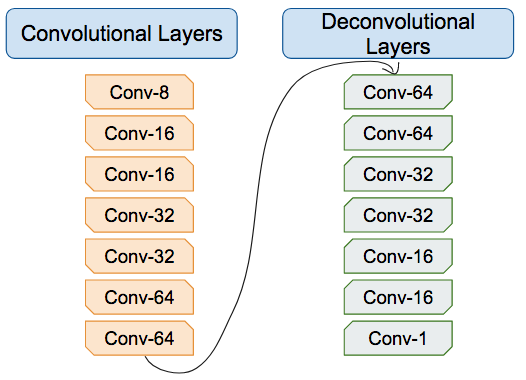
\includegraphics[width=0.5\textwidth]{Figure3}
\caption{Architecture of our CNN} \label{fig3}
\end{figure}

We used seven convolutional layers and a corresponding seven deconvolutional layers in our network. Each convolutional layer is followed by a dropout layer in order to avoid overfiting the data. There are two pooling layers, one between layers two and three and another between layers five and six. They are used to sample the data and reduce computation. As for the deconvolutional part, there are two upsample layers which use nearest neighbor interpolation. They lay between deconvolutional layers one and two, and layers five and six. \\

The main drawback of CNN is it mainly uses the shape information to detect lane. If there is a shadow in the road, it is generally unable to figure out where the lane is correctly.

\subsection{Recurrent Neural Network}

The Recurrent Neural Network uses the output of the CNN as its input. Its main goal is to make up for the previously stated drawback of the CNN. By using some previous knowledge, it is able to find the lane in some complex situations. The architecture of RNN model is shown below.

\begin{figure}[h]
\centering
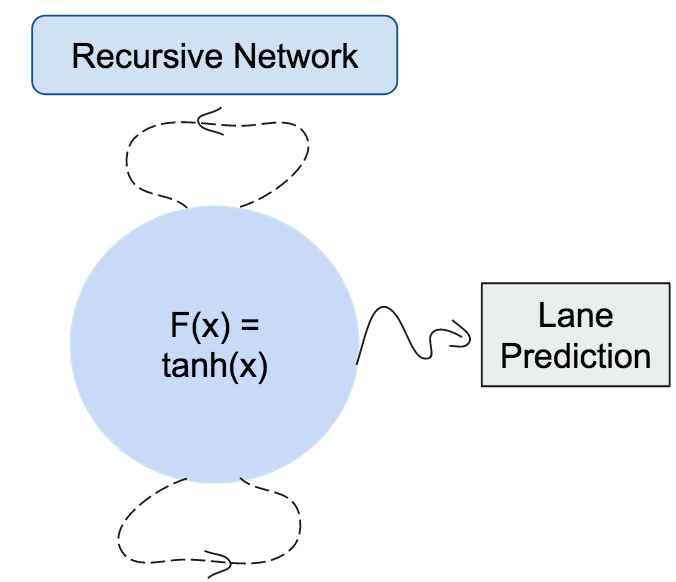
\includegraphics[width=0.5\textwidth]{Figure4}
\caption{Architecture of our CNN} \label{fig4}
\end{figure}

The main drawback of using a RNN is it will sometimes overtrust the memory. This will be more serious when the car is changing between lanes. Also, the RNN will sometimes has a delay in where it finds a lane because it needs its internal memory to be updated.

\section{Implementation}
All of our neural network implementation uses Tensorflow, a machine learning framework developed by Google~\cite{ref:11}. We use about 45000 labeled pictures from the CULane dataset to train our model.

\subsection{CNN Implementation}
In the CNN, we use 3 by 3 convolutional kernels with stride 1 by 1. The dropout rate is also set to 0.2. The filter number of each layer is directly labeled as in Fig \ref{fig3}. \\

In our network, the pooling layers and upsampling layer are corresponding. The pooling layers shrink the height of the data by a 2 by 2 window and the upsampling layer enlarges the height and width by two. Mean square error is used as the loss function and the optimizer is an Adam Optimizer.

\subsection{RNN Implementation}
We use a single layer of basic RNN cells which have 3200 neurons, using the sigmoid function as the activation function. Other type of cell like LSTM are not used because these cells maintain a much longer memory. This longer-term memory is unnecessary in lane detection problem because the lane location changes fast, and having long-term memory will result in serious overfitting problem.  Here, we shrink the image size to 40 * 80 once again so as to not exhaust our GPU's memory. After the prediction, output is enlarged proportionally to correspond with the output of our CNN. The RNN cells can memorize three frames and the training batch size is 17 frames. The memory size can be chosen according the refresh rate of the video. Mean square error is used as the loss function and the optimizer is an Adam Optimizer, which is same as our CNN.

\section{Evaluation}
In order to measure the effectiveness of our neural networks, we opted to generate confusion matrices based on the labeling output of the network. Specifically, we looked at the outputs of the combined RNN+CNN structure (Table \ref{tab:1}), and the outputs of just the CNN (Table \ref{tab:2}). All amounts are in pixels, out of 3200 pixels per image.

\setlength\tabcolsep{4pt}

\begin{table}[h]
\centering
\caption{RNN+CNN outputs Average Confusion Matrix}\label{tab:1}
\begin{tabular}{cccc}
\cline{3-4}
• & • & \multicolumn{2}{c}{Actual Class} \\
• & • & Lane & Non-Lane \\ 
\hline 
\multirow{2}{*}{Predicted Class} & Lane & 690.3 True Positives & 3039.7 False Positives \\ 
• & Non-Lane & 9.70 False Negatives & 9060.3 True Negatives \\ 
\hline 
\end{tabular} 
\end{table}

\begin{table}[H]
\centering
\caption{CNN outputs Average Confusion Matrix}\label{tab:2}
\begin{tabular}{cccc}
\cline{3-4}
• & • & \multicolumn{2}{c}{Actual Class} \\
• & • & Lane & Non-Lane \\ 
\hline 
\multirow{2}{*}{Predicted Class} & Lane & 418.2 True Positives & 38.7 False Positives \\ 
• & Non-Lane & 281.8 False Negatives & 12061 True Negatives \\ 
\hline 
\end{tabular} 
\end{table}

This analysis shows that the CNN is much more conservative with its lane assignments (stemming from the relatively low false-positive value for its outputs, compared to the outputs from the RNN). However, this conservative assignment pattern decreases the amount of true positives the network produces, when compared to the RNN output. The large false positive rate of the output from the RNN is probably due to the noise the network produces, as well as the network overfitting to the lane output. This could possibly corrected by employing dropout, or some kind of noise filtering on the inputs/outputs to the network.

\section{Summary}
Overall, our implementation of a combined Convolutional and Recurrent neural network did show signs of providing a solution to a serious problem in the field of lane detection in images. Specifically, by employing an RNN to take into account previous states, the network was found to be successful at maintaining a high degree of accuracy at lane-finding in challenging scenarios for just a CNN detector. There is much work that can be done on this system, however, and we have barely scratched the surface of what different architectures of neural networks can achieve in this field.

\section{Future Work}
For now, we have tested our system in static images and pre-taken videos, but the system would be expected to work in a real-time environment and thus we need more tests on how fast it can deal with the data. \\

Also, as we have shown in our evaluation part, the quality of our results from the recurrent neural network is decreased by a large amount of noise from the network and the network still fails to identify the lane well in some certain cases. Hence, future work can be done to find a way to filter out this noise. There are obviously many things we can try, such as changing the activation functions and applying thresholds to labeled images before sending it to the RNN network. \\

\section{Source Code}
All the source code for our neural network, as well as the data processing code, can be found in our GitHub Repository: \url{github.com/Spozder/LaneDetectionNNProject}
%
% ---- Bibliography ----
%
% BibTeX users should specify bibliography style 'splncs04'.
% References will then be sorted and formatted in the correct style.
%
% \bibliographystyle{splncs04}
% \bibliography{mybibliography}
%
\pagebreak
\begin{thebibliography}{8}
\bibitem{ref:1}
Chang, C., \& Lin, C. (2008, October 29). LIBSVM: a Library for Support Vector Machines. November 20, 2008.

\bibitem{ref:2}
Juan Pablo Gonzalez, Omit Ozguner. Lane Detection Using Histogram-Based Segmentation And Decision Trees. 2000 IEEE Intelligent Transportation Systems.

\bibitem{ref:3}
Sandipann P. Narote, Pradnya N. Bhujbal, Abbhilasha S. Narote, etc. A review of recent advances in lane detection and departure warning system. Pattern Recognition 73 (2018) 216–234.

\bibitem{ref:4}
Jun Li, Xue Mei, Danil Prokhorov, etc. Deep Neural Network for Structural Prediction and Lane Detection in Traffic Scene. IEEE TRANSACTIONS ON NEURAL NETWORKS AND LEARNING SYSTEMS, VOL. 28, NO. 3, MARCH 2017: 690-704.

\bibitem{ref:5}
Yan Tian, Judith Gelernter, Xun Wang, etc. Lane marking detection via deep convolutional neural network. Neurocomputing 280 (2018) 46–55.

\bibitem{ref:6}
Michael Virgo’s lane detection project description and source code: \\ \url{github.com/mvirgo/MLND-Capstone/tree/early\_steps}

\bibitem{ref:7}
Picture from Multimedia Laboratory, The Chinese University of Hong Kong: \\ \url{xingangpan.github.io/projects/CULane.html}

\bibitem{ref:8}
Vijay Badrinarayanan, Alex Kendall and Roberto Cipolla "SegNet: A Deep Convolutional Encoder-Decoder Architecture for Image Segmentation." PAMI, 2017.

\bibitem{ref:9}
OpenCV Library - \url{opencv.org/}

\bibitem{ref:10}
CULane Dataset - \url{xingangpan.github.io/projects/CULane.html}

\bibitem{ref:11}
Tensorflow Framework - \url{www.tensorflow.org/}


\end{thebibliography}

\pagebreak
\section{Individual Contributions}

\paragraph{Spencer Pozder}
Neural Network training, general neural network optimization, data analysis, analysis/summary sections of report \\

\paragraph{Yang Liu}
Data collection/labeling, data input/output, Introduction/Past Research/Dataset sections of report \\

\paragraph{Shen Chen}
Neural Network architecture, preliminary data input/output, Architecture/Implementation sections of report
\end{document}
